\documentclass[a4paper]{article}
\usepackage{amsfonts}
\usepackage{amsmath}
\usepackage{amssymb}
\usepackage{graphicx}     

\begin{document}
  
\noindent \large Auteur: Ahmed Meiyaki \\
\noindent \large Studierichting: Informatica\\
\noindent \large Oefeningenreeks 3G nr. 11.6\\

\medskip

\normalsize

$f(x) = \dfrac{x^2}{x-9} $\\

$\Rightarrow $ VA: $x = 9 $\\

$\lim\limits_{x\rightarrow 9+} f(x) = +\infty $\\

$\lim\limits_{x\rightarrow 9-} f(x) = -\infty $\\

$\Rightarrow$ HA: geen$ $\\

$SA: m = \lim\limits_{x \to \infty} \dfrac{f(x)}{x} = \lim\limits_{x \to \infty} \dfrac{x^2}{x^2 - 9x}  = 1$\\

$q = \lim\limits_{x \to \infty} \left(f(x) - x\right) = \lim\limits_{x \to \infty} \dfrac{x^2}{x - 9} - x$\\

$= \lim\limits_{x \to \infty} \dfrac{x^2}{x - 9} - \dfrac{x^2 - 9x}{x - 9} = \lim\limits_{x \to \infty} \dfrac{9x}{x - 9} = 9$\\

$\Rightarrow$ SA: $y = x + 9 $\\

Ligging:
\begin{tabular}{c|ccc}
	$x$ &     &   $9$   &   \\ \hline
		&  $-$  &   $/$   & $+$ \\
\end{tabular}

$x \rightarrow +\infty\Rightarrow f(x) > SA $\\

$x \rightarrow -\infty\Rightarrow f(x) < SA $\\

$f'(x) = \dfrac{2x\left(x-9\right) - x^2}{\left(x-9\right)^2} = \dfrac{2x^2 - 18x - x^2}{x^2 -18x + 81} $\\

$= \dfrac{x^2 - 18x}{\left(x - 9\right)^2} $\\

$f''(x) = \dfrac{\left(2x - 18\right)\left(x^2 - 18x + 81\right) - \left(x^2 -18x\right)\left(2x - 18\right)}{\left(x - 9\right)^4} $\\

$= \dfrac{\left(2x - 18\right)\left(x^2 - 18x + 81 - x^2 + 18x\right)}{\left(x - 9\right)^4} $\\

$= \dfrac{2\left(x - 9\right) \cdot 81}{\left(x - 9\right)^3} = \dfrac{162}{\left(x - 9 \right)^2} $\\



\begin{tabular}{c|ccccccccccc}
	$x$      &            &    $0$    &            &    $9$     &            &    $18$     &                     \\ \hline
	$f(x)$   &    $-$     &    $0$ 	  &   $-$      &    $|$     &   $+$      &    $+$     &    $+$          \\ \hline
	$f'(x)$  &    $+$     &    $0$    &   $-$      &    $|^{(2)}$     &   $-$      &    $0$     &    $+$           \\ \hline
	$f''(x)$ &    $-$     &    $-$    &   $-$      &    $|^{(3)$     &   $+$      &    $+$     &    $+$           \\ \hline
	& $\nearrow$ &  $M (0)$  & $\searrow$ & $|$ & $\searrow$ & $m(36)$ & $\searrow$ &         \\
	&    	 &    $\frown$        &    &   &    &  $\smile$  &    
\end{tabular}

Grafiek:
\begin{figure}[h]
	\centering
	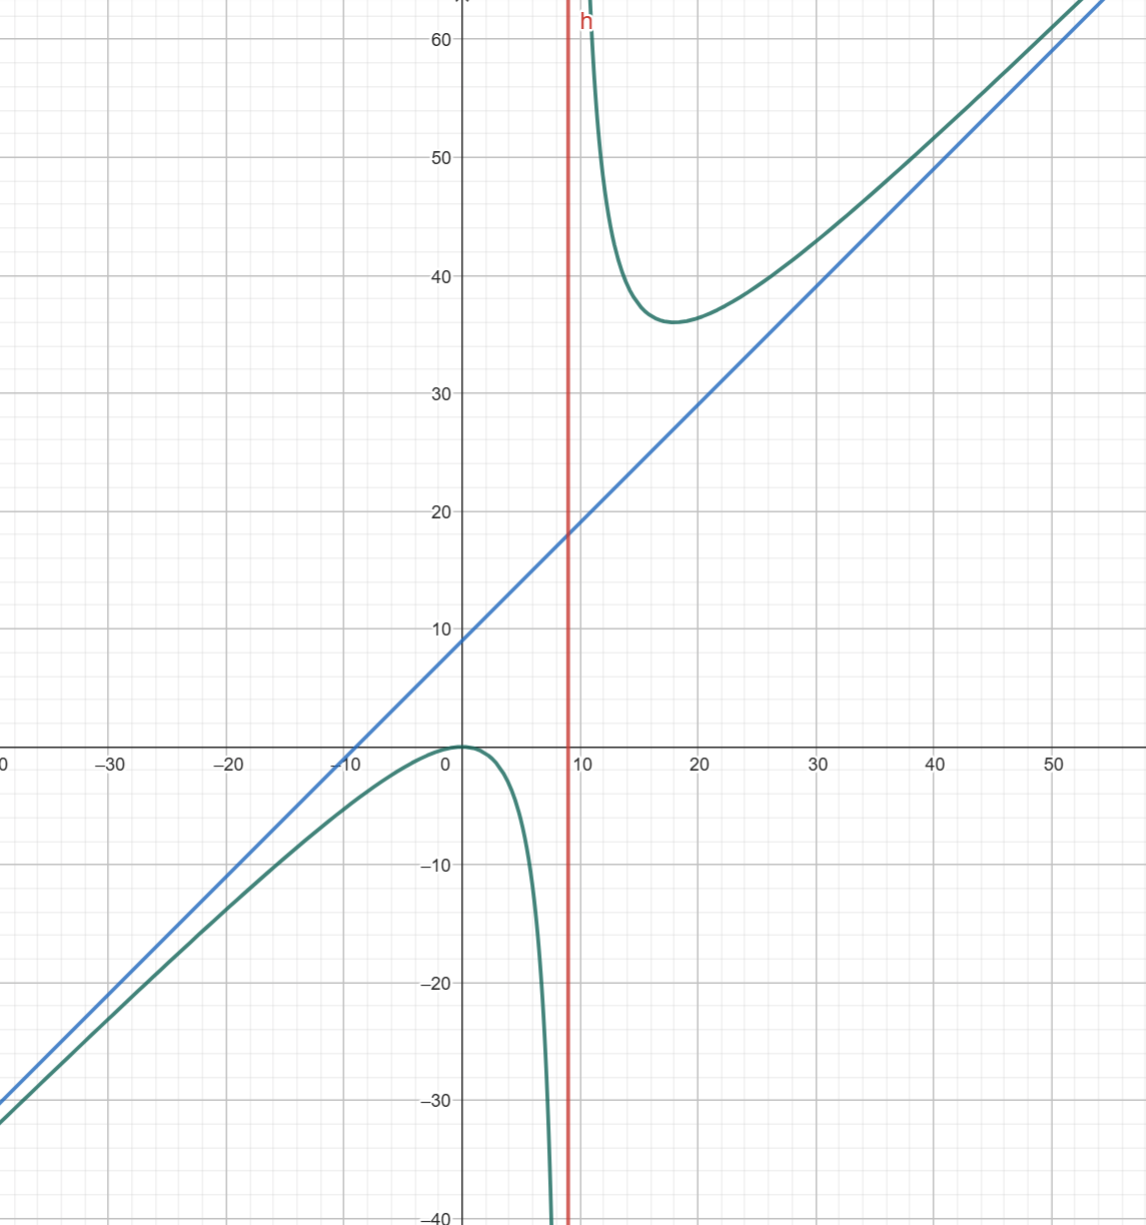
\includegraphics[width=8cm]{3G-11.6-ahmed.meiyaki.INF.png}
\end{figure}











\begin{thebibliography}{999}
%\bibitem{a} Referentie
\end{thebibliography}
\end{document} 
